\documentclass[10pt,a4paper,twocolumn,twoside]{article}
\usepackage[utf8]{inputenc}
\usepackage[catalan]{babel}
\usepackage{multicol}
\usepackage{graphicx}
\usepackage{fancyhdr}
\usepackage{times}
\usepackage{titlesec}
\usepackage{multirow}
\usepackage{lettrine}
\usepackage{hyperref}
\usepackage{enumitem}
\usepackage[top=2cm, bottom=1.5cm, left=2cm, right=2cm]{geometry}
\usepackage[figurename=Fig.,tablename=TAULA]{caption}
\captionsetup[table]{textfont=sc}

\author{\LARGE\sffamily Narcís Nogué Bonet}
\title{\Huge{\sffamily Aterratge autònom d'avions model basat en visió}}
\date{}

\newcommand\blfootnote[1]{%
  \begingroup
  \renewcommand\thefootnote{}\footnote{#1}%
  \addtocounter{footnote}{-1}%
  \endgroup
}

%
%\large\bfseries\sffamily
\titleformat{\section}
{\large\sffamily\scshape\bfseries}
{\textbf{\thesection}}{1em}{}

\begin{document}

\fancyhead[LO]{\scriptsize NARCÍS NOGUÉ BONET}
\fancyhead[RO]{\thepage}
\fancyhead[LE]{\thepage}
\fancyhead[RE]{\scriptsize ATERRATGE AUTÒNOM D'AVIONS MODEL BASAT EN VISIÓ}

\fancyfoot[CO,CE]{}

\fancypagestyle{primerapagina}
{
   \fancyhf{}
   \fancyhead[L]{\scriptsize TFG EN ENGINYERIA INFORMÀTICA, ESCOLA D'ENGINYERIA (EE), UNIVERSITAT AUTÒNOMA DE BARCELONA (UAB)}
   \fancyfoot[C]{\scriptsize Març de 2021, Escola d'Enginyeria (UAB)}
}

%\lhead{\thepage}
%\chead{}
%\rhead{\tiny EE/UAB TFG INFORMÀTICA: TÍTOL (ABREUJAT SI ÉS MOLT LLARG)}
%\lhead{ EE/UAB \thepage}
%\lfoot{}
%\cfoot{\tiny{February 2015, Escola d'Enginyeria (UAB)}}
%\rfoot{}
\renewcommand{\headrulewidth}{0pt}
\renewcommand{\footrulewidth}{0pt}
\pagestyle{fancy}

%\thispagestyle{myheadings}
\twocolumn[\begin{@twocolumnfalse}

%\vspace*{-1cm}{\scriptsize TFG EN ENGINYERIA INFORMÀTICA, ESCOLA D'ENGINYERIA (EE), UNIVERSITAT AUTÒNOMA DE BARCELONA (UAB)}

\maketitle

\thispagestyle{primerapagina}
%\twocolumn[\begin{@twocolumnfalse}
%\maketitle
%\begin{abstract}
\begin{center}
\parbox{0.915\textwidth}
{\sffamily
\textbf{Introducció--}
Com indica el títol, el meu Treball de Final de Grau consisteix en crear un
sistema de control autònom que sigui capaç d'aterrar un avió en una pista
d'aterratge utilitzant únicament una càmera i altres sensors bàsics com
acceleròmetres i giroscopis. Actualment la majoria de sistemes d'aterratge
autònom necessiten modificacions substancials de la pista d'aterratge per instal·lar
un sistema ILS (Instrument Landing System), dissenyat per permetre a una aeronau
aterrar de nit o en baixa visibilitat. Tot i així, hi ha un subgrup important dels
aeroports que segueixen les normes VFR (Visual Flight Rules), on només es pot
aterrar de dia i quan la visibilitat sigui suficient, ja que la única informació
que té el pilot és el contacte visual directe de la pista d'aterratge. La
majoria d'aeroports petits, aeròdroms i pistes de montanya cauen en aquesta categoria,
i per tant l'aterratge autònom per mètodes convencionals hi és de moment impossible.
La solució que proposo deriva directament d'aquesta restricció: si la majoria
de pistes d'aterratge estan pensades i dissenyades per a vol visual, un sistema
d'aterratge autònom ha de ser capaç d'aterrar de forma purament visual, i sense
confiar en cap input des de la pista d'aterratge, per a poder-se considerar plenament
autònom i genèric.
\\
%\end{abstract}
\\
}

{\vrule depth 0pt height 0.5pt width 4cm\hspace{7.5pt}%
\raisebox{-3.5pt}{\fontfamily{pzd}\fontencoding{U}\fontseries{m}\fontshape{n}\fontsize{11}{12}\selectfont\char70}%
\hspace{7.5pt}\vrule depth 0pt height 0.5pt width 4cm\relax}

\end{center}

\bigskip
\end{@twocolumnfalse}]

\blfootnote{$\bullet$ E-mail de contacte: nnogue4@gmail.com}
\blfootnote{$\bullet$ Menció realitzada: Computació}
\blfootnote{$\bullet$ Treball tutoritzat per: Felipe Lumbreras Ruiz (Department of Computer Science)}
\blfootnote{$\bullet$ Curs 2020/21}

\section{Objectius}

\lettrine[lines=3]{P}{er} la naturalesa del projecte, els objectius del meu Treball de Final de Grau poden
augmentar en complexitat molt ràpidament, i per tant els dividiré en dues seccions: els objectius necessàris per tenir un
MVP (Minimum Viable Product), i la resta d'objectius opcionals per seguir expandint el projecte més enllà.

Objectius per a un MVP:
\begin{itemize}
  \item Dissenyar i implementar un algoritme de control capaç d'aterrar un avió model si sap on és la pista d'aterratge.
  \item Dissenyar una simulació prou acurada d'un cas genèric d'aterratge, sobre la qual poder provar els algoritmes de control i de detecció de la pista.
  \item Dissenyar i implementar una xarxa neuronal capaç de reconèixer qualsevol pista d'aterratge sobre la qual hagi estat entrenada directament.
\end{itemize}
Objectius adicionals:
\begin{itemize}
\item Construïr un avió model capaç d'aterrar de forma autònoma a una pista d'aterratge.
\item Dissenyar i implementar una xarxa neuronal capaç de reconèixer qualsevol pista d'aterratge que no hagi vist prèvament.
\end{itemize}

\section{Estat de l'art}

En la introducció ja he parlat una mica de com funciona l'aterratge autònom avui en dia, en aquesta secció entraré més en detall
sobre els sistemes ILS i faré una ullada a altres projectes similars al meu i com han resolt els problemes que se'm presenten.

\subsection{El sistema ILS}
\label{subsec-ils-system}

El sistema ILS \cite{ILS}, anomenat Instrument Landing System o Sistema d'Aterratge Instrumental es considera un sistema d'ajuda per als pilots en situacions de baixa visibilitat, i només algunes categories d'ILS permeten aterratge automàtic a través
d'un sistema Autoland \cite{Autoland}.
Els sistemes ILS es poden classificar en tres categories: CAT I, CAT II i CAT III,
en funció de la precisió que proporcionen en el posicionament de l'aeronau, i només
les categories II i III es consideren suficients per a aterratges automàtics.

Pel que fa al funcionament, un ILS consisteix en dos transmissors de ràdio situats
a la pista d'aterratge. Un és el localitzador o \textit{localizer} (LOC), que 
indiquen la direcció de la pista (en la figura \ref{fig-ils-loc} es mostra la pista i la
senyal de ràdio vistes des de sobre).


% Per a fer que la figura ocupi les dues columnes utilitzeu "figure*" per comptes de "figure"
\begin{figure}[!h]
\centering
\fbox{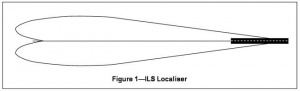
\includegraphics[width=0.4\textwidth, trim={0.2cm 0.5cm 0.2cm 0.1cm}, clip]{img/ILS-LOC}}
	\caption{Rà dio localitzador ILS}
	\label{fig-ils-loc}
\end{figure}

L'altra ràdio és la de pendent de descens o \textit{Glide-Scope} (GS), que permet a
l'aeronau controlar la ràtio de descens durant l'aproximació. (la figura \ref{fig-ils-gs} mostra la
pista d'aterratge i la senyal de ràdio vistes de perfil).

\begin{figure}[!h]
\centering
\fbox{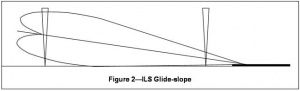
\includegraphics[width=0.4\textwidth, trim={0.2cm 0.5cm 0.2cm 0.1cm}, clip]{img/ILS-GS}}
	\caption{Ràdio Glide-Scope ILS}
	\label{fig-ils-gs}
\end{figure}

El sistema ILS funciona bé i és molt robust, però necessita que les antenes de ràdio
a la pista estiguin instal·lades i funcionin correctament, i avui en dia només els
aeroports i aeròdroms amb més transit solen tenir aquest sistema, les pistes més petites i els aeròdroms en llocs remots solen quedar fora de l'equació pel que fa a aterratges
amb ILS.

\subsection{Un altre exemple de subsecció}
\label{subsec-exemple2}

La taula \ref{tab:senzilla} és un exemple de taula senzilla. En canvi, la taula \ref{tab:taula2} és més completa.

Hi ha moltes referències \textit{on-line} de \LaTeX, com.

% Utilitzeu el begin table només en cas de vole taules flotants. Si les voleu al lloc, tabular directament.
\begin{table}
\caption{Taula d'exemple}
\label{tab:senzilla}
\begin{center}
\begin{tabular}{|c|c|}
\hline
One & Two\\
\hline
Three & Four\\
\hline
\end{tabular}
\end{center}
\end{table}



\begin{table}
\caption{Taula més completa}
\label{tab:taula2}

\begin{center}
\begin{tabular}{ |l|l|l| }
\hline
\multicolumn{3}{ |c| }{Team sheet} \\
\hline
Goalkeeper & GK & Paul Robinson \\ \hline
\multirow{4}{*}{Defenders} & LB & Lucus Radebe \\
 & DC & Michael Duburry \\
 & DC & Dominic Matteo \\
 & RB & Didier Domi \\ \hline
\multirow{3}{*}{Midfielders} & MC & David Batty \\
 & MC & Eirik Bakke \\
 & MC & Jody Morris \\ \hline
Forward & FW & Jamie McMaster \\ \hline
\multirow{2}{*}{Strikers} & ST & Alan Smith \\
 & ST & Mark Viduka \\
\hline
\end{tabular}
\end{center}
\end{table}

\section{Planificació}

En aquesta secció desciuré la planificació que vull seguir durant tot el
projecte i el procés que he seguit per arribar-hi a través del mètode
PERT \cite{PERT}.

\subsection{Work Breakdown Structure}
Començaré amb l'Estructura Detallada de Treball o Work Breakdown Structure (WBS)
\cite{WBS}. En la següent llista organitzaré les tasques que considero que són 
necessàries en una estructura jeràrquica de dos nivells:

\begin{enumerate}
    \item Planificar el projecte de forma detallada.
    \item Investigar possibles solucions pel problema plantejat.
    \begin{enumerate}[label*=\arabic*.]
        \item Recopilar una llista de possibles solucions (models de xarxa neuronal).
        \item Investigar pros i contres de cada possible solució
        \item Escollir models a implementar, poden ser més d'un si vull investigar-ne més d'un en profunditat
    \end{enumerate}
    \item Implementar solucions escollides per a una única pista d'aterratge
    \begin{enumerate}[label*=\arabic*.]
        \item Crear datasets o simulació simple per a l'entrenament no supervisat.
        \item Implementar l'algoritme d'entrenament de les solucions escollides.
        \item Provar cada xarxa neuronal i iterar fins aconseguir la precisió desitjada.
    \end{enumerate}
    \item Implementar una simulació complexa per provar el sistema.
    \begin{enumerate}[label*=\arabic*.]
        \item Investigar possibles formes de fer una simulació.
        \item Implementar la simulació de terreny.
        \item Implementar la simulació de l'avió model.
    \end{enumerate}
    \item Provar el sistema sobre la simulació.
    \begin{enumerate}[label*=\arabic*.]
        \item Integrar lògica de control sobre la simulació.
    \end{enumerate}
    \item Investigar integració arduino amb hardware tipic d'avions radiocontrol.
    \item Construir un avió model pathfinder.
    \begin{enumerate}[label*=\arabic*.]
        \item Investigar sobre construcció d'avions model.
        \item Construir estructura principal.
        \item Construir electrònica del model.
        \item Proves inicials de vol.
    \end{enumerate}
    \item Construir avió model definitiu, de zero o extenent el model pathfinder.
    \begin{enumerate}[label*=\arabic*.]
        \item Construir estructura principal.
        \item Construir electrònica del model.
        \item Integrar el hardware de control autònom al model.
    \end{enumerate}
    \item Implementar xarxa neuronal i controls en el model.
    \item Provar el model sobre una pista d'aterratge real.
    \begin{enumerate}[label*=\arabic*.]
        \item Sobrevolar la pista controlant l'avió manualment i recopilar les dades necessàries per a poder analitzar les decisions del model després del vol.
        \item Provar l'estabilitat de vol en ràfagues curtes de vol autònom.
        \item Provar aproximacions autònomes i prendre control just abans de l'aterratge.
        \item Provar un aterratge complet.
    \end{enumerate}
    \item Ampliar la xarxa neuronal perquè l'avió pugui aterrar en qualsevol aeroport.
\end{enumerate}


\subsection {Assignació de temps per tasca (PERT)}

\begin{table}
\caption{Assignació de temps (en hores)}
\label{tab:taulaTemps}

\begin{center}
\begin{tabular}{ |c|c|c|c|c| }
\hline
     & To & Tn & Tp & T$\gamma$ \\ \hline
     1   & 5  & 8  & 10 &    \\ \hline
     \hline
     2.1 & 1  & 2  & 3  & 2  \\ \hline
     2.2 & 3  & 5  & 8  &    \\ \hline
     2.3 & 1  & 1  & 2  &    \\ \hline
     \hline
     3.1 & 5  & 8  & 12 &    \\ \hline
     3.2 & 8  & 10 & 15 &    \\ \hline
     3.3 & 10 & 12 & 18 &    \\ \hline
     \hline
     4.1 & 2  & 3  & 5  &    \\ \hline
     4.2 & 3  & 4  & 6  &    \\ \hline
     4.3 & 5  & 6  & 8  &    \\ \hline
     \hline
     5.1 & 2  & 3  & 5  &    \\ \hline
     \hline
     6   & 3  & 5  & 8  &    \\ \hline
     \hline
     7.1 & 3  & 5  & 8  &    \\ \hline
     7.2 & 5  & 6  & 8  &    \\ \hline
     7.3 & 5  & 6  & 8  &    \\ \hline
     7.4 & 4  & 5  & 7  &    \\ \hline
     \hline
     8.1 & 2  & 3  & 5  &    \\ \hline
     8.2 & 2  & 3  & 5  &    \\ \hline
     8.3 & 4  & 5  & 8  &    \\ \hline
     \hline
     9   & 6  & 8  & 12 &    \\ \hline
     \hline
    10.1 & 5  & 8  & 12 &    \\ \hline
    10.2 & 5  & 8  & 12 &    \\ \hline
    10.3 & 5  & 8  & 12 &    \\ \hline
     \hline
     11 & 10 & 15 & 25 &    \\ \hline
\end{tabular}
\end{center}
\end{table}

\section{Conclusions}

.... ..  .... .. .... ... ..... ... ..... ... ... ..... .... .
.... ..  .... .. .... ... ..... ... ..... ... ... ..... .... .
.... ..  .... .. .... ... ..... ... ..... ... ... ..... .... .
.... ..  .... .. .... ... ..... ... ..... ... ... ..... .... .
.... ..  .... .. .... ... ..... ... ..... ... ... ..... .... .
.... ..  .... .. .... ... ..... ... ..... ... ... ..... .... .
.... ..  .... .. .... ... ..... ... ..... ... ... ..... .... .
.... ..  .... .. .... ... ..... ... ..... ... ... ..... .... .
.... ..  .... .. .... ... ..... ... ..... ... ... ..... .... .
.... ..  .... .. .... ... ..... ... ..... ... ... ..... .... .
.... ..  .... .. .... ... ..... ... ..... ... ... ..... .... .
.... ..  .... .. .... ... ..... ... ..... ... ... ..... .... .
.... ..  .... .. .... ... ..... ... ..... ... ... ..... .... .
.... ..  .... .. .... ... ..... ... ..... ... ... ..... .... .

\section*{Agraïments}

... ..  .... .. .... ... ..... ... ..... ... ... ..... .... .
.... ..  .... .. .... ... ..... ... ..... ... ... ..... .... .
.... ..  .... .. .... ... ..... ... ..... ... ... ..... .... .
.... ..  .... .. .... ... ..... ... ..... ... ... ..... .... .
.... ..  .... .. .... ... ..... ... ..... ... ... ..... .... .

\begin{thebibliography}{9}
\bibitem{ILS}
Instrument Landing System (ILS)
\\\url{https://www.skybrary.aero/index.php/Instrument_Landing_System_(ILS)}
\\Visitat 28-2-2021

\bibitem{Autoland}
Autoland Systems
\\\url{https://www.skybrary.aero/index.php/Autoland}
\\Visitat 1-3-2021

\bibitem{PERT}
La metodologia PERT
\\\url{https://en.wikipedia.org/wiki/Program_evaluation_and_review_technique}
\\Visitat 1-3-2021

\bibitem{WBS}
Work Breakdown Structure
\\\url{https://www.workbreakdownstructure.com/}
\\Visitat 1-3-2021

\end{thebibliography}

\end{document}

© 2021 GitHub, Inc.
Terms
Privacy
Security
Status
Docs
Contact GitHub
Pricing
API
Training
Blog
About
